\documentclass[]{scrartcl}

\usepackage{graphicx}
%%\usepackage{amsmath}

\usepackage{natbib}

%opening
\title{PHY 982 - HW 1}
\author{Xingze Mao \\ Zachary Matheson \\ Thomas Redpath}
\date{}

\begin{document}

\maketitle

Beryllium-11 is a one-neutron halo nucleus with 4 protons and 7 neutrons. According to the shell model, we would expect 2 neutrons in a $1s_{1/2}$ state, 4 in $1p_{3/2}$, and the seventh neutron in a $1p_{1/2}$ state. Experimentally, we find that the ground state of $^{11}$Be is a $2s_{1/2}$ state with the valence neutron bound by roughly 500 keV. This is explained by looking at the evolution of single particle levels across the $N=7$ isotones (Figure~\ref{fig:n7isotones}). For the more neutron rich isotones, the  $2s_{1/2}$ state drops below the $1p_{1/2}$. This reordering of the energy levels has been attributed to residual effective two-body interactions as pointed out by Talmi and Unna \citep{TalmiUnna1960} who explained the inversion of these two levels by considering the interaction of the valence neutron with the protons in the $1p_{3/2}$ shell. 

\begin{figure}
\centering
	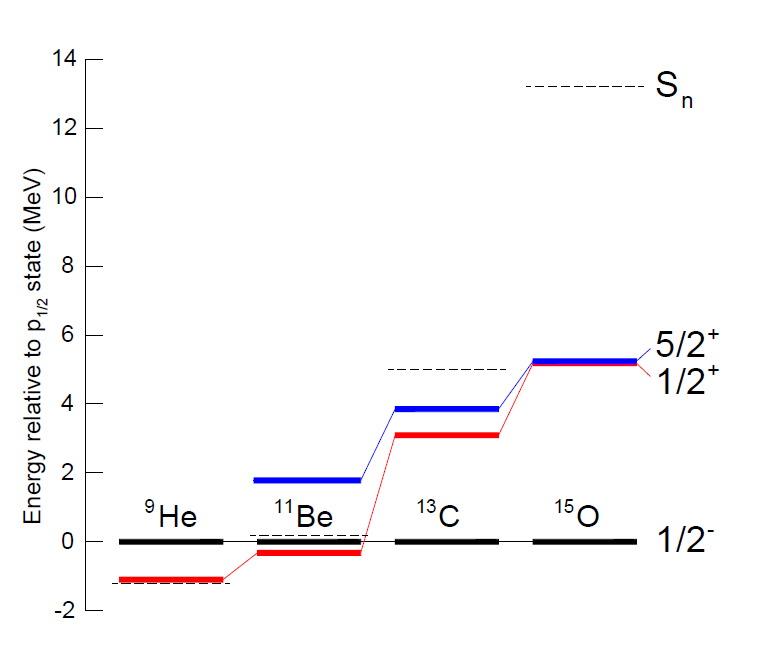
\includegraphics[width=\textwidth]{figures/n7isotones.png}
	\caption{The evolution of single particl levels for the $N=7$ isotones (from \citep{Schmitt2011}). It is clear that the $1/2 ^+$ state drops below the $1/2 ^-$ in energy for $^{11}$Be.}
	\label{fig:n7isotones}
\end{figure}



%which is certainly related to the fact that $^{11}$Be is a halo nucleus and not a truly bound state $\leftarrow$ \textit{\textbf{Is it correct to say that halo nuclei are not "truly bound"? And is this a sufficient answer?}} . . . halo nuclei are considered bound - Be-11's ground state is bound by 0.5 MeV and its first excited by 0.18 MeV

Slightly above the ground state in energy we find the $1/2^-$ state we otherwise might have expected to be the ground state, and above that is the $5/2^+$ state that follows according to the shell model. After that, things start to diverge from shell model predictions, but up to this point, the system behaves almost like one would expect via the shell model except for the ground state.

\section*{Method}\nonumber

Solving the radial scattering equations involves finding a solution to Schr\"{o}dinger's equation (eq.~\ref{eq:seq}) numerically out to a range where the interaction between the neutron and the $^{10}$Be becomes negligible.

\begin{equation}
	u_{L} '' (R) = f(R) u_{L} (R)
	\label{eq:seq}
\end{equation}
where,
\begin{equation}
	f(R) = \frac{2 \mu}{\hbar ^2} (V(R) - E) + \frac{L(L+1)}{R^2}
\end{equation}
with $V(R)$ replaced by the Woods-Saxon potential
\begin{equation}
	V(R) = \frac{ V_0 }{ 1 + \exp{ \frac{ R - R_{\mathrm{ws}} }{a_{\mathrm{ws}}}}}
	\label{eq:ws}
\end{equation}

\noindent The resulting wavefunction must then be matched to the asymptotic form of the solution (eq.~\ref{eq:asym}).
\begin{equation}
	\chi _L ^{ext} (R) = A _L [ H _L ^- (0,R) - S_L H_L ^+ (0,R) ]
	\label{eq:asym}
\end{equation}

\begin{equation}
	H_L ^{\pm} (R) = G_L (R) \pm i F_L (F)
\end{equation}
where $F_L (R)$ and $G_L (R)$ are the spherical Bessel functions times $R$.

The matching involves equating the logarithmic derivative of the numerically determined interior wavefunction to that of the exterior asymptotic wavefunction. Since the interior wavefunction is computed numerically, its logarithmic derivative can be used to compute the R-matrix element (eq.~\ref{eq:rmtx}) and, subsequently, the S-matrix element for a given value of $L$.


\begin{equation}
	\mathbf{R}_L = \frac{1}{a} \frac{u _L (a)}{u _L ' (a)} = \frac{1}{a} \frac{H^- - \mathbf{S}_L H^+}{H'^- - \mathbf{S}_L H' ^+}
	\label{eq:rmtx}
\end{equation}

\subsection*{Numerical Integration}

We performed the numerical integration of eq.~\ref{eq:seq} using the Runge-Kutta method implemented in a Python program (outlined in the following section). Application of the Runge-Kutta method requires writing the second-order differential equation as coupled first-order equations $y(R)$ and $w(R) = y'(R)$. This allows us to apply the method to each first order equation and find the wavefunction and its derivative over the region of interaction.

The Runge-Kutta method solves a first order DE iteratively. For a known $y(R)$, the desired $y(R+h)$ may be approximated:

\begin{equation}
	y(R+h) \approx y(R) + h \sum_{i=1}^N \omega_i y'(R + \nu_i h,y(R + \nu_ih))
	\label{eq:rkaprx}
\end{equation}
where $h$ is some small step size and primes denote differentiation with respect to R. Let $\nu_i =0$ so that the first term in the sum becomes $k_1 = h y' (R,y(R))$ - this is known from the initial conditions and the DE describing how $y'$ depends on $y$. Now use $k_1$ to approximate the second term $k_2 = h y' (R+\alpha h, y(R) + \beta k_1)$. Now, eq.~\ref{eq:rkaprx} may be written

\begin{equation}
	y(R+h) \approx y(R) + \omega_1 k_1 + \omega_2 k_2
	\label{eq:rk1}
\end{equation}
Taylor expanding the LHS of eq.~\ref{eq:rk1}, substituting for $k_{1,2}$ and denoting $y'$ as $f$

\begin{equation}
	hf + \frac{h^2}{2} \left ( f' + f \frac{df}{dy} \right ) = \omega_1 hf + \omega_2 \left  ( hf + \alpha h^2 f' + \beta h^2 f \frac{df}{dy} \right )
	\label{eq:rk2}
\end{equation}
Equate coefficients of $hf,f',f df/dy$ to constrain $\alpha, \beta, \omega_{1,2}$. A higher order, more accurate Runge-Kutta formula is produced by keeping more terms in the sum from eq.~\ref{eq:rkaprx} and going to higher order in the Taylor expansion of the LHS of eq.~\ref{eq:rk1} to determine the constants. For our code, we use fourth order Runge-Kutta.

\subsection*{Python Code}

The python code we wrote to compute the radial wavefunctions and phase shifts follows the basic outline:

\begin{enumerate}
	\item Define the matching radius, $L$ value, step size, and physical parameters
	\item Set initial conditions ($y_0 = 0, y_0 ' = 1.0$) 
	\item Define functions to compute $f(R)u_L(R)$ (from eq.~\ref{eq:seq}), the Hankel functions (in terms of the cylindrical Bessel functions) and their derivatives
	\item Create an array to hold values of the wavefunction and its derivative at each step along our grid out to the matching radius
	\item Apply the Runge-Kutta formula to populate the array
	\item Compute $\mathbf{S}_L$ from the matching condition
	\item Apply this routine for a range of energies to plot phase shift versus energy
\end{enumerate}

%\clearpage

\section*{Wavefunction plots}

Figures~\ref{fig:e01l0} - \ref{fig:e01l2} plot the real and imaginary parts of the radial wavefunctions for $l=0,1,2$ and $E=0.1$ MeV. Figures~\ref{fig:e30l0} - \ref{fig:e30l2} plot the wavefunctions for $l=0,1,2$ and $E=3.0$ MeV. The point in each plot where the line changes from solid to dashed is the matching point.

%% E = 0.1 MeV
\begin{figure}[h]
\centering
	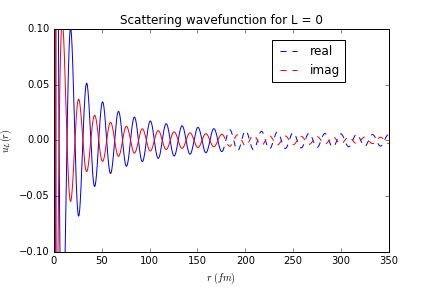
\includegraphics[width=0.75\textwidth]{figures/E01/l0.png}
	\caption{The real (blue) and imaginary (red) parts of the radial wavefunction for $E = 0.1$ MeV and $l=0$.}
	\label{fig:e01l0}
\end{figure}

\begin{figure}
\centering
	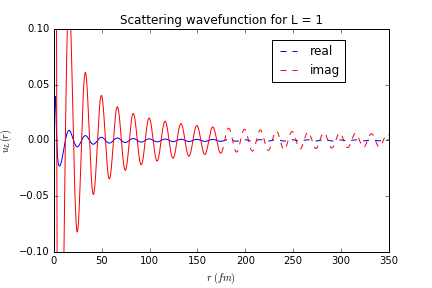
\includegraphics[width=0.75\textwidth]{figures/E01/l1.png}
	\caption{The real (blue) and imaginary (red) parts of the radial wavefunction for $E = 0.1$ MeV and $l=1$.}
	\label{fig:e01l1}
\end{figure}

\begin{figure}
\centering
	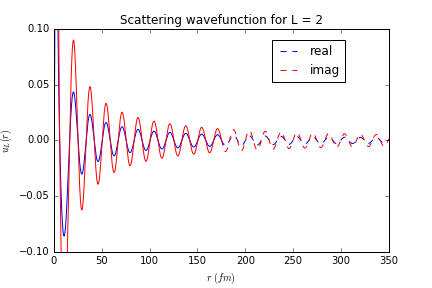
\includegraphics[width=0.75\textwidth]{figures/E01/l2.png}
	\caption{The real (blue) and imaginary (red) parts of the radial wavefunction for $E = 0.1$ MeV and $l=2$.}
	\label{fig:e01l2}
\end{figure}


%% E = 3.0 MeV
\begin{figure}
\centering
	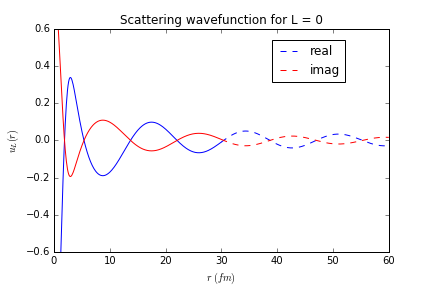
\includegraphics[width=0.75\textwidth]{figures/E30/l0.png}
	\caption{The real (blue) and imaginary (red) parts of the radial wavefunction for $E = 3.0$ MeV and $l=0$.}
	\label{fig:e30l0}
\end{figure}

\begin{figure}
\centering
	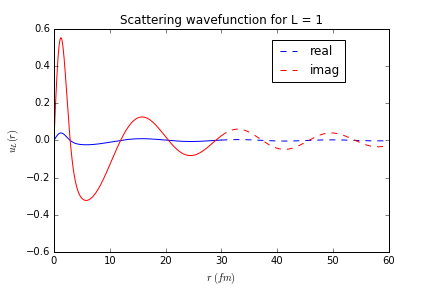
\includegraphics[width=0.75\textwidth]{figures/E30/l1.png}
	\caption{The real (blue) and imaginary (red) parts of the radial wavefunction for $E = 3.0$ MeV and $l=1$.}
	\label{fig:e30l1}
\end{figure}

\begin{figure}[h]
\centering
	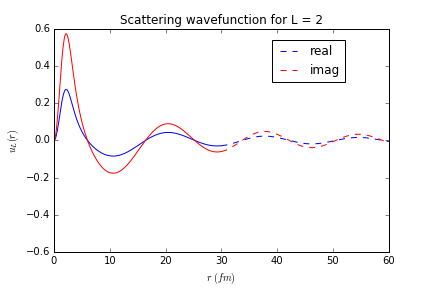
\includegraphics[width=0.75\textwidth]{figures/E30/l2.png}
	\caption{The real (blue) and imaginary (red) parts of the radial wavefunction for $E = 3.0$ MeV and $l=2$.}
	\label{fig:e30l2}
\end{figure}


\section*{Phase Shifts and Resonances}

Figure~\ref{fig:phase} plots the phase shifts $\delta(E)$ for $l=0,1,2$ over the energy range $[0.1,4.0]$ MeV. A weak resonance appears for $l=2$ around $E=1.5$ MeV. We estimate the width by approximating the slope of the sharply rising region of the $\delta (E)$ curve to be $\sim 260$ keV. In terms of the $^{11}$Be continuum structure, this could be interpreted as the $5/2 ^+$ second excited state which has a measured energy of 1.8 MeV and width of 100 keV. This second excited state energy less the 500 keV $S _n $ for $^{11}$Be is close to our calculated ``resonance'' energy, though our estimated width is larger by a factor of 2.

\begin{figure}
\centering
	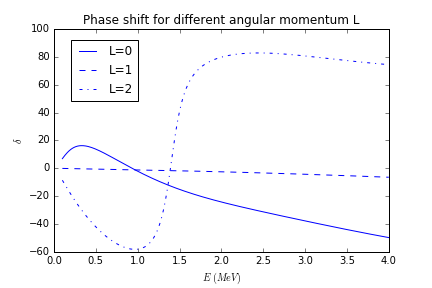
\includegraphics[width=0.85\textwidth]{figures/phase.png}
	\caption{Phase shifts $\delta(E)$ for $l=0,1,2$. A weak resonance appears for $l=2$ near $E=1.4$ MeV with a width of $\sim 260$ keV.}
	\label{fig:phase}
\end{figure}

\clearpage

%\begin{table}
%\centering
%	\begin{tabular}{ c | c | c }
%	$l$ & $\delta (E) $ & $\Gamma$ [MeV]\\
%\hline
%	0 & & \\
%	1 & & \\
%	2 & & \\
%	\end{tabular}
%	\caption{

%%\bibliographystyle{apj}
\bibliographystyle{plain}
\bibliography{ref}

\end{document}
